% ====================================================================
%  PROYECTO FINAL -- Computacion Paralela y Distribuida (CS4052)
%  Proyecto #7: Redes Neuronales -- Entrenamiento paralelo de MLP
%  Compila con:  tectonic informe_final.tex   (o pdfLaTeX/XeLaTeX)
% ====================================================================
\documentclass[11pt,a4paper]{article}

% ---------- Codificacion e idioma ----------
\usepackage[utf8]{inputenc}
\usepackage[T1]{fontenc}
\usepackage[spanish,es-nolists,es-tabla,es-noindentfirst]{babel}
\usepackage[a4paper,margin=2.3cm]{geometry}

% ---------- Tipografia elegante (Palatino-like) ----------
\usepackage{newpxtext}
\usepackage{newpxmath}
\usepackage{microtype}        % micro-ajustes tipograficos

% ---------- Matematicas, tablas, graficos ----------
\usepackage{amsmath}
\usepackage{booktabs}
\usepackage{graphicx}
\usepackage{algorithm}
\usepackage{algpseudocode}

% ---------- Color (solo grises) ----------
\usepackage{xcolor}

% ---------- Cajas destacadas ----------
\usepackage{tcolorbox}
\tcbuselibrary{breakable,skins}
\newtcolorbox{nota}[1][]{
  enhanced, colback=black!3, colframe=black!45, boxrule=0.4pt, arc=2pt,
  left=8pt, right=8pt, top=5pt, bottom=5pt, breakable,
  fonttitle=\bfseries, coltitle=white,
  attach boxed title to top left={xshift=6pt, yshift=-2pt},
  boxed title style={colback=black!70, arc=1pt, boxrule=0pt},
  #1}

% ---------- Posicion fija de figuras ----------
\usepackage{float}

% ---------- Estilo de secciones (subrayado fino, todo negro) ----------
\usepackage{titlesec}
\titleformat{\section}
  {\Large\bfseries}{\thesection}{0.6em}{}
  [\vspace{3pt}{\titlerule[0.8pt]}]
\titleformat{\subsection}
  {\large\bfseries}{\thesubsection}{0.5em}{}
\titleformat{\subsubsection}
  {\normalsize\bfseries}{\thesubsubsection}{0.4em}{}
\titlespacing*{\section}{0pt}{1.3ex plus 0.4ex}{0.7ex}
\titlespacing*{\subsection}{0pt}{1ex plus 0.3ex}{0.5ex}

% ---------- Hipervinculos (sin color) ----------
\usepackage[hidelinks]{hyperref}

\setlength{\parskip}{6pt}\setlength{\parindent}{0pt}
\linespread{1.15}

% ====================================================================
\begin{document}

% ---------- Encabezado del documento ----------
\begin{center}
\vspace*{0.3cm}
{\Large\bfseries Proyecto Final}\\[0.2cm]
{\large Paralelización del entrenamiento de múltiples MLP con distintas semillas}\\[0.15cm]
{\normalsize Computación Paralela y Distribuida (CS4052) -- 2026-I}\\[0.45cm]
Kalos Lazo \quad Aaron Navarro \quad Fernando Usurin\\[0.1cm]
{\small Participación: 100\% cada uno (contribución equitativa)}\\[0.1cm]
{\small Profesor: José Fiestas}\\[0.1cm]
{\small Julio de 2026}
\end{center}
\rule{\textwidth}{0.4pt}
\vspace{0.2cm}

% ====================================================================
\section{Introducción}

El proyecto consiste en paralelizar el entrenamiento de un conjunto de
perceptrones multicapa (MLP) entrenados con distintas semillas aleatorias,
conservando el de mayor exactitud sobre el conjunto de prueba. Dado que la
inicialización de pesos depende de la semilla del generador pseudoaleatorio,
una práctica robusta es entrenar varios modelos y conservar el mejor
\cite{lecun2015,goodfellow2016}.

Este procedimiento es \textbf{embarazosamente paralelo}: cada entrenamiento es
independiente y los procesos solo se sincronizan al final para comparar
exactitudes y seleccionar el mejor \cite{farias2023}. Es por ello un caso ideal
para un modelo PRAM de \textbf{memoria compartida}.

\textbf{Solución planteada.} A partir del Algoritmo~1 (entrenamiento secuencial de
múltiples MLP) proponemos:
\begin{enumerate}
  \item Un algoritmo PRAM sobre el modelo CREW que reparte el conjunto de
        semillas $S=\{0,\dots,p_s-1\}$ entre $p$ procesadores y aplica una
        reducción final \emph{arg\-máx} en árbol.
  \item Una implementación en Python con \texttt{scikit-learn}
        \cite{pedregosa2011,buitinck2013}, paralelizada con
        \texttt{multiprocessing} (análogo a OpenMP \cite{dagum1998,chapman2007}).
  \item Una caracterización empírica de tiempo, speedup, eficiencia y GFLOP/s
        para $p\in\{1,2,4,8,16,32\}$ y $n\in\{5\,000,\dots,40\,000\}$, con
        superposición de la curva teórica y análisis de escalabilidad
        (strong scaling bajo Amdahl \cite{amdahl1967,hill2008} y weak scaling bajo
        Gustafson \cite{gustafson1988}).
\end{enumerate}

% ====================================================================
\section{Método}

\subsection{Algoritmo secuencial de referencia}
El Algoritmo~1 entrena $p_s$ modelos MLP, uno por cada semilla, y conserva el de
mayor exactitud.

\begin{algorithm}[H]
\caption{Entrenamiento secuencial de múltiples MLP con distintas semillas}
\label{alg:seq}
\begin{algorithmic}[1]
\Require Datos $(X,y)$, semillas $S=\{0,\dots,p_s{-}1\}$, hiperparámetros $(\alpha,\eta,h,T_{\max})$
\Ensure Modelo $M^\ast$ con mayor exactitud
\State Dividir $(X,y)$ en train/test \Comment{una sola vez}
\State $A_{\text{best}}\gets -\infty$;\; $M^\ast\gets \emptyset$
\ForAll{$s\in S$}
  \State inicializar RNG con semilla $s$;\; construir y entrenar $M_s$
  \State $A_s\gets \mathrm{accuracy}(M_s,X_{\text{test}},y_{\text{test}})$
  \If{$A_s>A_{\text{best}}$} $A_{\text{best}}\gets A_s$;\; $M^\ast\gets M_s$ \EndIf
\EndFor
\State \Return $M^\ast$
\end{algorithmic}
\end{algorithm}

\subsection{Algoritmo PRAM propuesto (CREW, memoria compartida)}
\label{sec:pram}

Asumimos un PRAM \textbf{CREW} con $p$ procesadores que comparten memoria global:
varios procesadores leen concurrentemente el dataset y los hiperparámetros, pero
las escrituras se serializan mediante una reducción \emph{arg\-máx}
\cite{bennun2019}. Cada $P_k$ trabaja sobre el subconjunto de semillas $S_k$, con
$|S_k|\approx\lceil p_s/p\rceil$ (reparto balanceado). Conviene precisar una
cuestión de modelo: en el informe parcial, la lectura de datos se denominó
\emph{``Broadcast''}, lo cual es impropio de la memoria compartida ---allí los
datos residen en memoria global y cada procesador simplemente los \emph{lee} de
forma concurrente (acceso CREW), sin necesidad de difundirlos---. Por ello se ha
renombrado a \textbf{lectura concurrente} y, atendiendo la observación del
docente, no se contabiliza como un paso paralelo independiente.

\begin{algorithm}[H]
\caption{PRAM-CREW: entrenamiento de múltiples MLP (memoria compartida)}
\label{alg:pram}
\begin{algorithmic}[1]
\Require $(X,y)$, $S=\{0,\dots,p_s{-}1\}$, $p$ procesadores, hiperparámetros
\Ensure $M^\ast$ con mayor exactitud
\Statex \textcolor{black!55}{/* Paso 1 -- Split (secuencial). NO se mide */}
\State Dividir $(X,y)$; \textbf{dejar} todo en memoria compartida
\Statex \textcolor{black!55}{/* Paso 2 -- Entrenamiento local (\textbf{pardo}) */}
\ForAll{$k=0,\dots,p-1$ \textbf{pardo}} \Comment{$W_2=O(p_s\,E\,n\,d\,h)$, $P_2=p$}
  \State $P_k$ \textbf{lee} de memoria compartida $(X_{\text{train}},\dots)$ \Comment{CREW}
  \State entrenar las MLP de $S_k$; guardar mejor $(A^{(k)}_{\text{best}}, M^{(k)})$ local
\EndFor
\Statex \textcolor{black!55}{/* Pasos 3\,..\,$2{+}\log_2 p$ -- Reducción arg\-máx en árbol */}
\For{$\text{stride}=1,2,4,\dots,p/2$} \Comment{$\text{stride}\gets 2\cdot\text{stride}$ cada ronda}
  \ForAll{$k=0,\,2\cdot\text{stride},\,4\cdot\text{stride},\dots$ \textbf{pardo}}
    \If{$A^{(k+\text{stride})}_{\text{best}}>A^{(k)}_{\text{best}}$}
       $A^{(k)}_{\text{best}}\gets A^{(k+\text{stride})}_{\text{best}}$;\; $M^{(k)}\gets M^{(k+\text{stride})}$
    \EndIf
  \EndFor
\EndFor
\State \Return $M^\ast=M^{(0)}$
\end{algorithmic}
\end{algorithm}

\textbf{Nota de implementación.} La reducción \emph{arg\-máx} en árbol de
$\log_2 p$ rondas es el \emph{modelo} PRAM que justifica el término $\log_2 p$
del costo (Sección~\ref{sec:metricas}); en la implementación, la reducción se
realiza con un \texttt{max} serial sobre los $p_s$ resultados durante la fase
\emph{join} del esquema \emph{fork--join}. Ambas variantes producen el mismo
$M^\ast$ y su diferencia es despreciable en la práctica, pues la reducción mide
$\le 3.6\%$ del tiempo total (Sección~\ref{sec:resultados}).

\subsection{Justificación del uso de memoria compartida}
\label{sec:just}

\begin{enumerate}
  \item \textbf{Comunicación mínima.} Es un esquema embarazosamente paralelo:
        la única interacción es la reducción \emph{arg\-máx} final (árbol de
        $\log_2 p$ rondas). No se aprovecha nada del paso de mensajes.
  \item \textbf{Datos compartidos y de solo lectura.} Cada MLP se entrena con
        todo el dataset. En memoria compartida basta con que los $p$
        procesadores \emph{lean} las mismas referencias (herencia por
        \texttt{fork}); en memoria distribuida habría que copiar el dataset a
        cada proceso (memoria $\times p$). La memoria compartida es aquí más
        eficiente.
  \item \textbf{Modelo de programación.} Se usa \texttt{multiprocessing} de
        Python como análogo de OpenMP \cite{dagum1998,chapman2007}: patrón
        \emph{fork--join} donde los trabajadores heredan la memoria global y se
        sincronizan al recolectar resultados. El GIL de Python impide hilos
        reales, de ahí el uso de procesos.
\end{enumerate}

\subsection{Métricas y modelo de costo}
\label{sec:metricas}

A partir del Algoritmo~\ref{alg:pram} se obtiene el modelo de costo que permite,
por un lado, predecir el comportamiento esperado del paralelo y, por otro,
contrastarlo con las mediciones de la Sección~\ref{sec:resultados}. La
descomposición paso a paso (paradigma \emph{Work--Time}) asocia a cada etapa su
trabajo $W_i$ y el número de procesos activos $P_i$:

\begin{center}\small
\begin{tabular}{llll}
\toprule
Paso & Descripción & $W_i$ & $P_i$ \\\midrule
1 & Split y carga en memoria compartida & $O(n)$ & 1 \\
2 & Entrenamiento de $\lceil p_s/p\rceil$ MLP (\textbf{pardo}) & $O(p_s\,E\,n\,d\,h)$ & $p$ \\
$3\dots$ & Reducción arg\-máx ($\log_2 p$ rondas) & $O(p)$ & $p/2,\dots,1$ \\
final & Escritura de $M^\ast$ & $O(1)$ & 1 \\
\bottomrule
\end{tabular}
\end{center}

El entrenamiento de los $p_s$ modelos domina el trabajo total,
$W = O(p_s\,E\,n\,d\,h)$, que coincide con el tiempo secuencial $T_s$: la
paralelización \emph{no añade trabajo}, únicamente lo redistribuye entre
procesadores. El camino crítico (span) queda fijado por \emph{un único}
entrenamiento, $T_\infty = O(E\,n\,d\,h)$, y define el límite inferior del tiempo,
por muchos procesadores que se asignen. Combinando ambas cotas mediante el
Teorema de Brent se obtiene el modelo de costo
\begin{equation}\label{eq:tp}
\boxed{\,T_p \;\approx\; a\,\frac{p_s}{p}\,E\,n\,d\,h \;+\; b\,\log_2 p\,,}
\end{equation}
donde $a$ es una \textbf{constante empírica} que traduce la complejidad
estructural $E\,n\,d\,h$ a segundos (refleja la velocidad de la máquina) y $b$ un
\textbf{overhead empírico por ronda} que agrupa la sincronización \emph{fork--join}
y la contención de memoria; conviene subrayar que $b$ \emph{no} es la latencia de
la reducción \emph{arg\-máx} propiamente dicha, cuyo peso medido es $\le 3.6\%$ de
$T_{\text{total}}$ (Sección~\ref{sec:resultados}). Ambas se estiman
por mínimos cuadrados en la Sección~\ref{sec:teorica}. Conviene recalcar que
$a$ y $E\,d\,h$ son factores de naturaleza distinta: $E\,d\,h$ es la complejidad
del MLP (fija), mientras que $a$ depende del hardware.

De (\ref{eq:tp}) se desprende que el speedup tiende a $S(p)\to p$ cuando el
término de cómputo domina, comportamiento que la experimentación deberá
confirmar. Asimismo, el costo $C_p = T_p\cdot p$ resulta $O(W)$ mientras
$p \le W/T_\infty = O(p_s)$; como todos los experimentos cumplen $p\le p_s=32$,
el reparto de semillas aprovecha los procesadores sin dejarlos ociosos, esto es,
el algoritmo es WT-óptimo.

Finalmente, el costo en operaciones de un MLP
($\mathrm{FLOPs}=4\,E\,h\,(d+c)\,n$, forward+backward) habilita el reporte del
rendimiento en GFLOP/s, métrica con la que se caracteriza además la saturación
del hardware.

% ====================================================================
\section{Resultados y análisis}
\label{sec:resultados}

\subsection{Configuración experimental}
\textbf{Plataforma:} cluster HPC \textbf{Khipu} de UTEC, nodo \texttt{n003}
(Intel Xeon Gold 6130, 32 núcleos lógicos $\approx$ 16 físicos con
hyper-threading, 224\,GB DDR4), gestionado con Slurm.
\textbf{Software:} Python 3.11, scikit-learn 1.9, numpy. \textbf{Hiperparámetros:}
$p_s=32$ semillas, $d=32$ features, $h=128$ neuronas, $c=10$ clases, $E=100$
épocas, $\alpha=10^{-4}$, $\eta=10^{-3}$. El BLAS se limita a 1 hilo por proceso
(\texttt{OMP\_NUM\_THREADS=1}) para que la única paralelización sea la nuestra.
Cada punto $(n,p)$ se mide con 2 repeticiones; se reporta el \textbf{worker
crítico} (máximo entre procesos), sin incluir la lectura ni el split. El código
es determinista: la versión paralela reproduce exactamente las 32 exactitudes y
el mismo modelo ganador que la secuencial.

\subsection{Tiempos de ejecución}
\begin{figure}[H]\centering
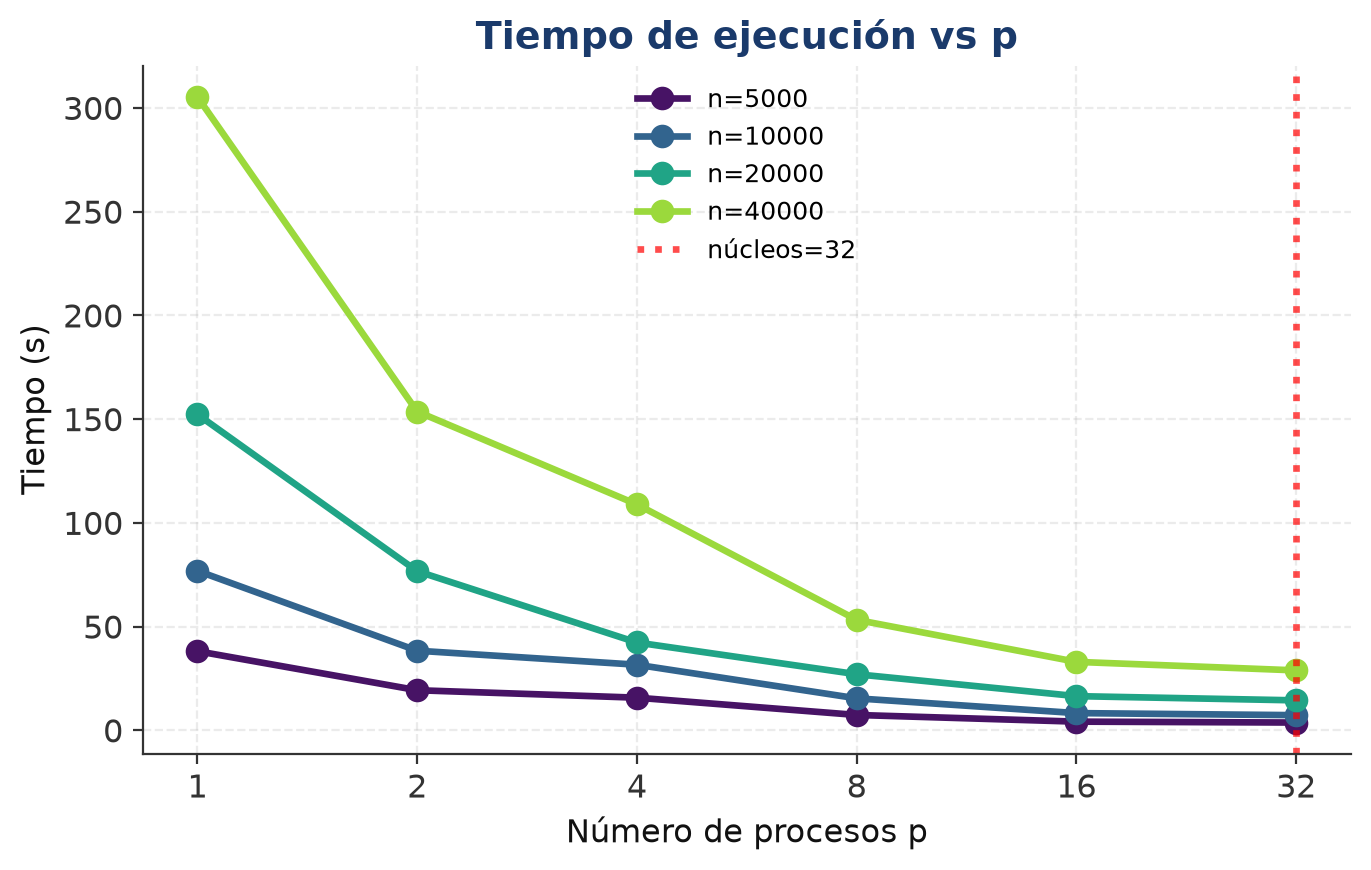
\includegraphics[width=0.72\textwidth]{../figures/fig_khipu_tiempos.png}
\caption{Tiempo vs $p$ (Khipu, 32 núcleos). La reducción $T_{\text{reduce}}$ es
$\le 3.6\%$ (y $<1\%$ para $n$ grande): el cuello no es la comunicación.}
\end{figure}

El tiempo cae con $p$ sin saturarse prematuramente. La reducción
$T_{\text{reduce}}$ es $\le 3.6\%$ de $T_{\text{total}}$ (y $<1\%$ para $n$
grande), confirmando el carácter embarazosamente paralelo.

\subsection{Speedup}
\begin{figure}[H]\centering
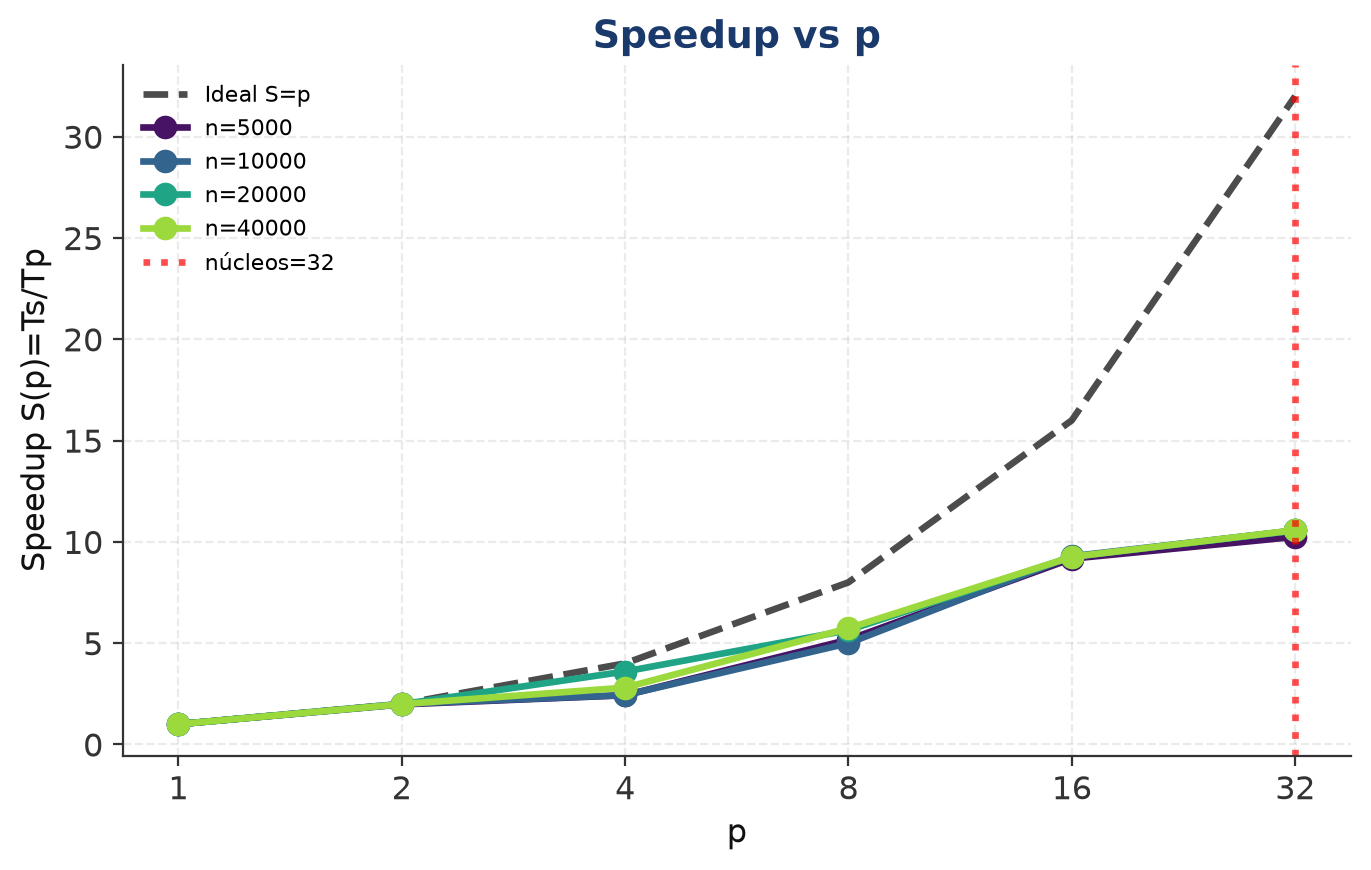
\includegraphics[width=0.72\textwidth]{../figures/fig_khipu_speedup.png}
\caption{Speedup $S(p)=T_s/T_p$ vs $p$ frente a la cota ideal $S=p$.}
\end{figure}

El modelo de costo de la Sección~\ref{sec:metricas} anticipa un speedup cercano
a $p$ mientras el cómputo domine sobre la reducción. La Figura confirma esa
predicción en la región baja: $S(p)$ sigue la diagonal ideal hasta $p\approx 2$
($E\approx0.99$) y conserva una eficiencia razonable ($E\approx0.6$--$0.9$ según
$n$) hasta $p\approx 8$, lo que valida tanto el reparto de semillas como la
hipótesis de trabajo dominante. Se observa una anomalía puntual en $p=4$ ---con
eficiencia incluso inferior a la de $p=8$ para los $n$ pequeños y varianza alta
entre repeticiones---, atribuible a efectos de turbo-boost/NUMA con pocos
procesos activos. Más allá de $p\approx 8$ el crecimiento se atenúa y
se estabiliza en torno a $S\approx 10.6$ para $p=32$. Este techo, muy por debajo
de los 32 núcleos lógicos del nodo, no obedece a la comunicación
($T_{\text{reduce}}\le 3.6\%$) sino a dos factores del hardware: el
\textbf{hyper-threading} presenta 32 núcleos lógicos que en realidad son
$\approx 16$ físicos, acotando el speedup real al intervalo $[10,16]$; y la
\textbf{contención del ancho de banda de memoria}, propia de una carga
\emph{memory-bound}, desacelera cada MLP desde $\sim$9.6\,s (aislado) hasta
$\sim$28.9\,s cuando 32 procesos compiten por la memoria. El siguiente análisis
de eficiencia permite cuantificar cuánto de ese techo se traduce en
aprovechamiento real.

\subsection{Eficiencia}
\begin{figure}[H]\centering
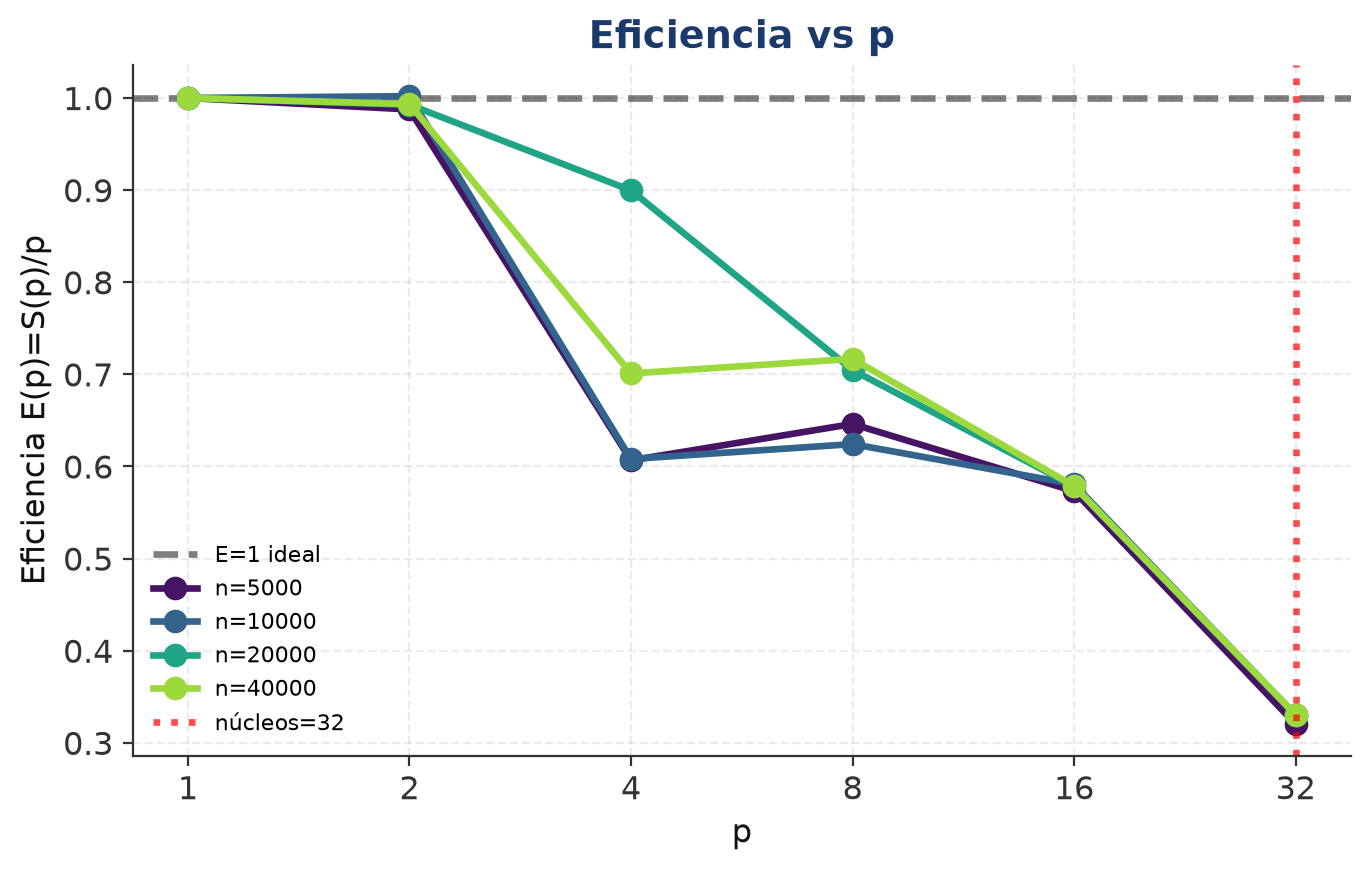
\includegraphics[width=0.72\textwidth]{../figures/fig_khipu_eficiencia.png}
\caption{Eficiencia $E(p)=S(p)/p$ vs $p$.}
\end{figure}

La eficiencia es la contraparte informativa del speedup: mide cuánto aporta cada
procesador adicional. Bajo \emph{strong scaling} decrece con $p$ ---de forma no
estrictamente monótona, por el bache en $p=4$ ya señalado---, pasando de
$\sim$0.99 en $p=2$ a $\sim$0.33 en $p=32$, reflejando los mismos
límites identificados arriba (hyper-threading y contención). Esta degradación es
mucho más modesta bajo \emph{weak scaling} (Sección~\ref{sec:weak}), donde la
carga por procesador se conserva: aunque tampoco es perfecta ---la naturaleza
\emph{memory-bound} del MLP se hace sentir al crecer el problema---, la pérdida
de eficiencia es claramente inferior. En consecuencia, la eficiencia \textbf{no
es constante} en escalabilidad fuerte, y se preserva bastante mejor en
escalabilidad débil. Resta verificar si el modelo teórico reproduce este
comportamiento.

\subsection{Validación frente a la complejidad teórica}
\label{sec:teorica}
\begin{figure}[H]\centering
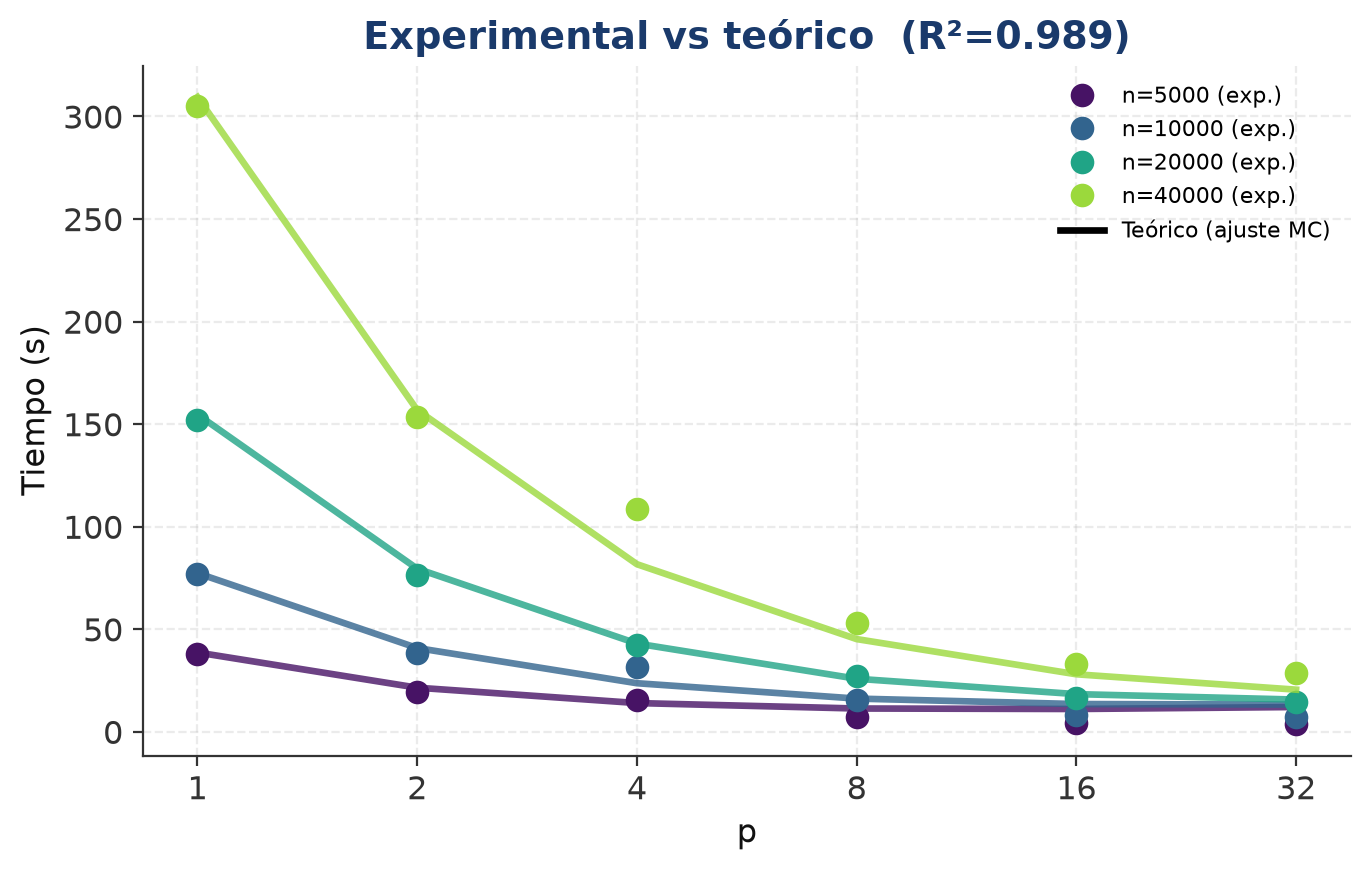
\includegraphics[width=0.72\textwidth]{../figures/fig_khipu_teorica.png}
\caption{Tiempo experimental (puntos) frente a la curva teórica de la
Ec.~(\ref{eq:tp}) ajustada por mínimos cuadrados no-negativos (líneas).}
\end{figure}

Para contrastar el modelo de costo con la realidad se ajustó la
Ec.~(\ref{eq:tp}) por mínimos cuadrados no-negativos sobre los 48 puntos
experimentales. El ajuste arroja $R^2=\textbf{0.989}$, con
$a\approx\textbf{$5.9\times 10^{-10}$}$\,s y $b=\textbf{2.18}$\,s. Como muestra
la Figura, el término dominante $a\,(p_s/p)\,E\,n\,d\,h$ reproduce fielmente la
región lineal, mientras que el término $b\,\log_2 p$ (con $b\approx2.18$\,s) no
representa la reducción \emph{arg\-máx} ---cuyo peso medido es $\le 3.6\%$ de
$T_{\text{total}}$--- sino que absorbe empíricamente el overhead de sincronización
y la contención de memoria a alto $p$ que el término lineal no captura. El elevado $R^2$ permite concluir que la expresión
teórica ---que, a diferencia del parcial, \textbf{incluye el término $\log_2 p$}
de la reducción--- constituye una descripción correcta del costo del algoritmo.

\subsection{Rendimiento (GFLOP/s)}
\begin{figure}[H]\centering
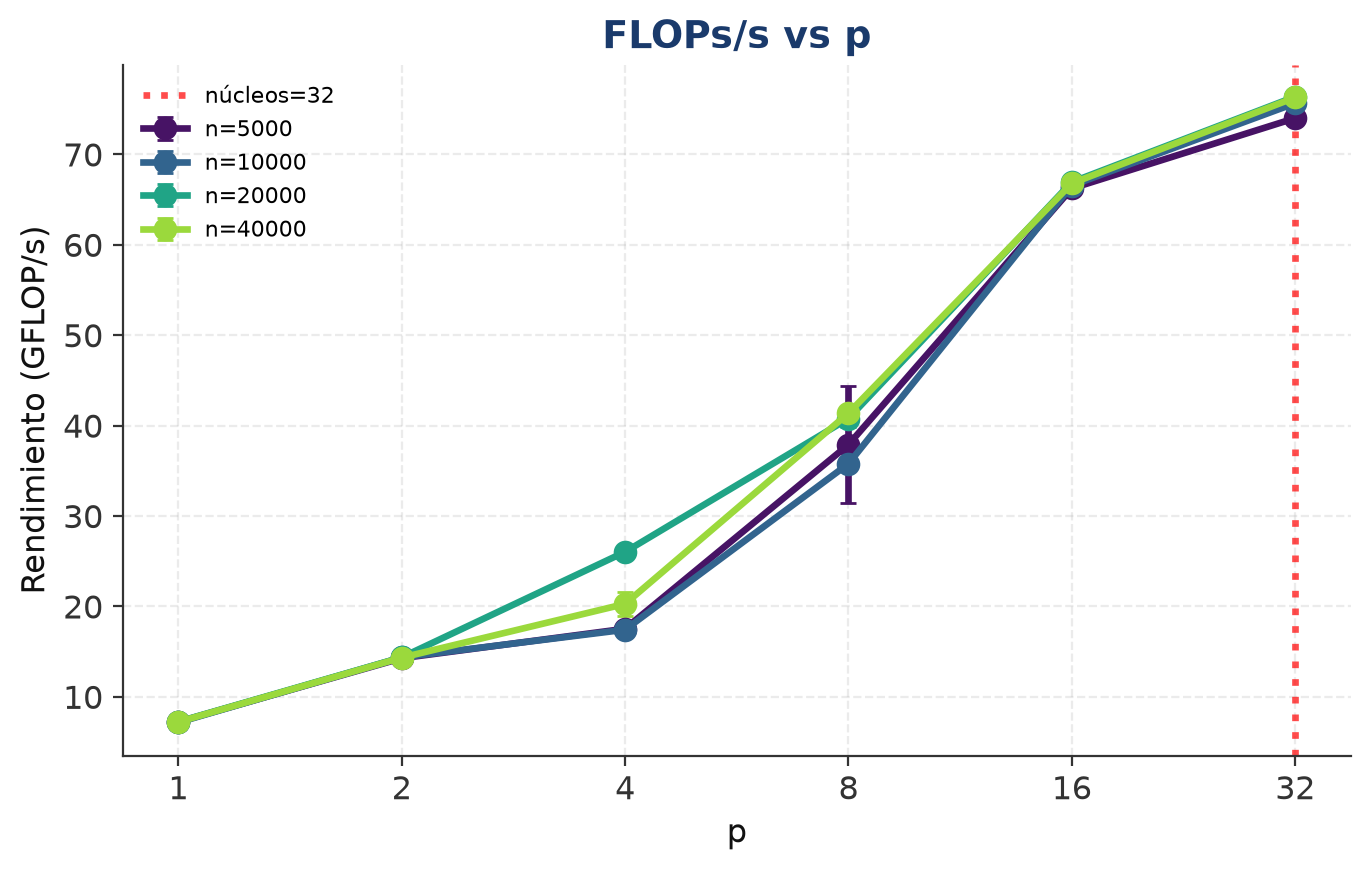
\includegraphics[width=0.72\textwidth]{../figures/fig_khipu_gflops.png}
\caption{Rendimiento (GFLOP/s) vs $p$.}
\end{figure}

El rendimiento complementa la lectura del speedup desde la óptica de las
operaciones: crece de forma sostenida hasta $\sim$67 GFLOP/s en $p=16$ y
\textbf{$\sim$76 GFLOP/s} en $p=32$. Que la curva se sature al mismo nivel
que el speedup, y no siga escalando con $p$, confirma que el cuello final no son
los núcleos sino el ancho de banda de memoria compartido. Los dos análisis
siguientes caracterizan ambos regímenes de escalabilidad para cerrar esta
interpretación.

\subsection{Escalabilidad fuerte}
\begin{figure}[H]\centering
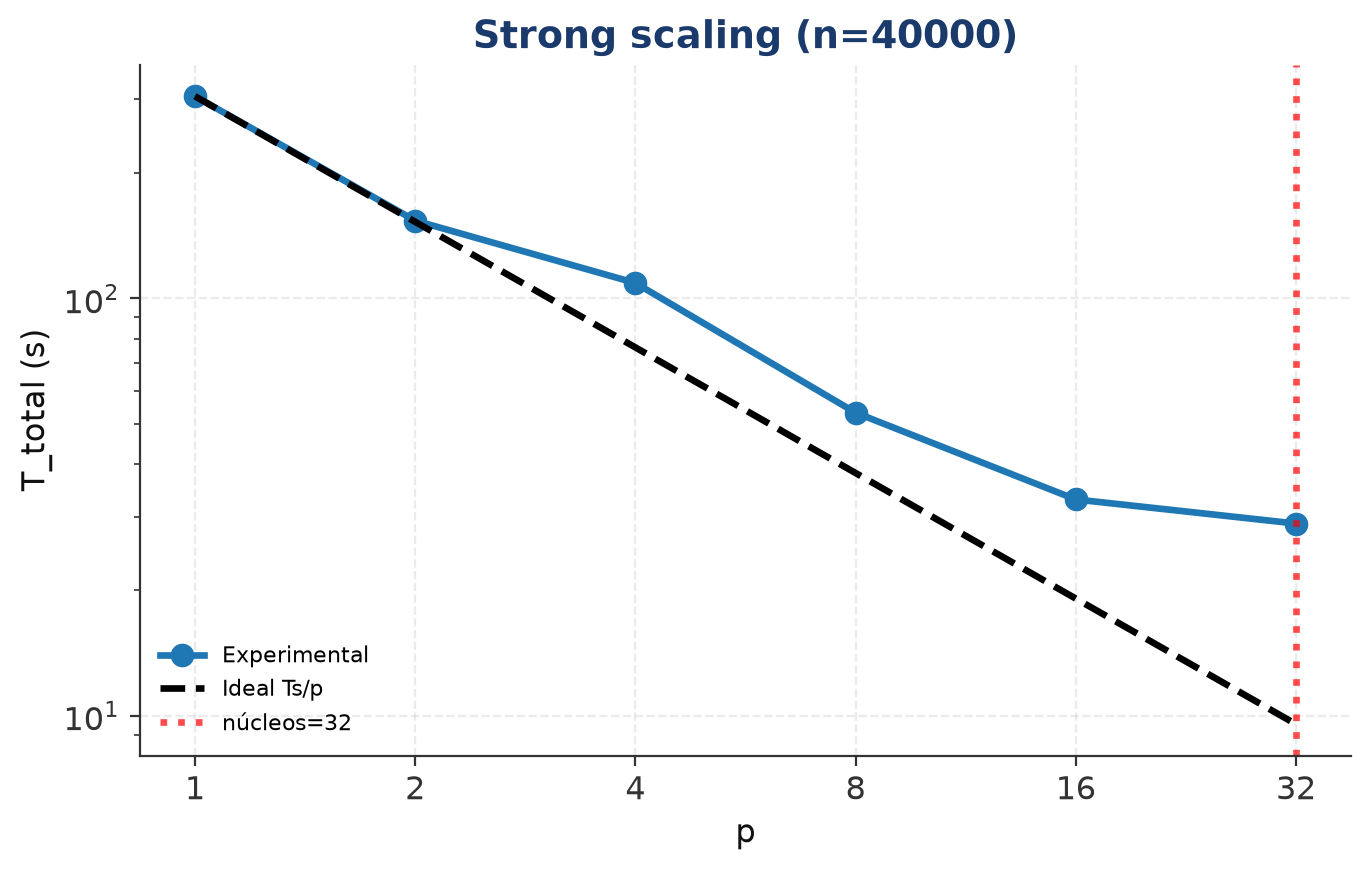
\includegraphics[width=0.62\textwidth]{../figures/fig_khipu_strong.png}
\caption{Strong scaling para $n=40000$ (log--log): la pendiente sigue $1/p$ hasta
$p\approx 8$ y luego se aplana.}
\end{figure}

Con el tamaño del problema fijo, la complejidad empírica sigue $T_p\propto 1/p$
en la región lineal, confirmando el costo $\Theta(E\,n\,d\,h)$ por procesador
derivado en la Sección~\ref{sec:metricas}. El aplanamiento posterior es la
signature del límite por ancho de banda ya identificado. Este régimen, sin
embargo, es el más exigente; conviene examinar el comportamiento cuando el
problema crece junto con $p$.

\subsection{Escalabilidad débil}
\label{sec:weak}
\begin{figure}[H]\centering
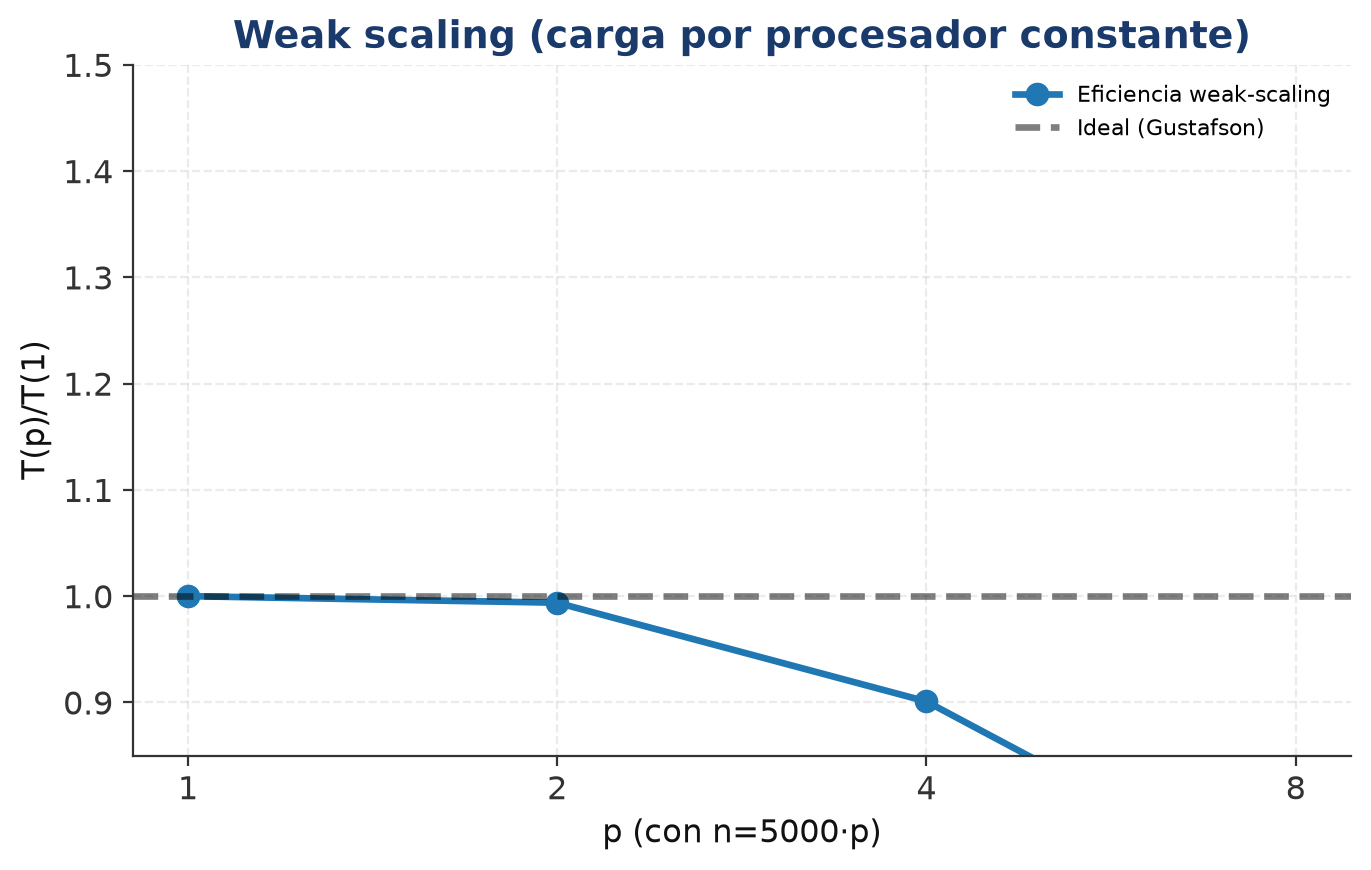
\includegraphics[width=0.62\textwidth]{../figures/fig_khipu_weak.png}
\caption{Weak scaling con $n=5000\cdot p$: la cercanía a $1$ indica escalabilidad
ideal bajo Gustafson.}
\end{figure}

Bajo weak scaling ($n$ crece proporcionalmente con $p$) el cociente
$T(p)/T(1)$ se mantiene cercano a la unidad en los primeros pasos y luego crece
moderadamente, hasta $\approx$1.4 en $p=8$: aunque cada procesador conserva su
carga nominal, el mayor tamaño total del problema intensifica la contención de
memoria. Esta degradación es, no obstante, claramente inferior a la del strong
scaling, lo que confirma que el algoritmo aprovecha mejor los recursos cuando el
problema crece junto con ellos, en línea con la ley de Gustafson.

\subsection{Mejoras propuestas}
El análisis anterior sugiere varias líneas de mejora. La contención de memoria a
alto $p$ podría aliviarse con una \textbf{asignación dinámica} de semillas que
balancee MLPs de duración heterogénea. El techo impuesto por Python invita a un
\textbf{backend nativo OpenMP/C++} que elimine el overhead de proceso, y a
explotar un \textbf{segundo nivel de paralelismo dentro del MLP} (BLAS multihilo
o GPU) debidamente coordinado con el de semillas. Finalmente, escalar a un nodo
de \textbf{128 núcleos} permitiría verificar el comportamiento más allá del
rango explorado.

\subsection{Tabla resumen}
\begin{center}\small
\begin{tabular}{rrrrrrr}
\hline
n & p & $T_{total}$ (s) & Speedup & Eficiencia & GFLOP/s & best-acc \\
\hline
5000 & 1 & 38.11 & 1.00 & 1.000 & 7.2 & 0.765 \\
5000 & 2 & 19.30 & 1.98 & 0.988 & 14.3 & 0.765 \\
5000 & 4 & 15.71 & 2.43 & 0.607 & 17.5 & 0.765 \\
5000 & 8 & 7.37 & 5.17 & 0.646 & 37.9 & 0.765 \\
5000 & 16 & 4.16 & 9.17 & 0.573 & 66.2 & 0.765 \\
5000 & 32 & 3.72 & 10.25 & 0.320 & 74.0 & 0.765 \\
10000 & 1 & 76.85 & 1.00 & 1.000 & 7.2 & 0.798 \\
10000 & 2 & 38.35 & 2.00 & 1.002 & 14.4 & 0.798 \\
10000 & 4 & 31.60 & 2.43 & 0.608 & 17.4 & 0.798 \\
10000 & 8 & 15.39 & 4.99 & 0.624 & 35.8 & 0.798 \\
10000 & 16 & 8.27 & 9.29 & 0.581 & 66.5 & 0.798 \\
10000 & 32 & 7.28 & 10.56 & 0.330 & 75.7 & 0.798 \\
20000 & 1 & 152.25 & 1.00 & 1.000 & 7.2 & 0.856 \\
20000 & 2 & 76.68 & 1.99 & 0.993 & 14.4 & 0.856 \\
20000 & 4 & 42.31 & 3.60 & 0.900 & 26.0 & 0.856 \\
20000 & 8 & 27.01 & 5.64 & 0.705 & 40.8 & 0.856 \\
20000 & 16 & 16.45 & 9.26 & 0.578 & 66.9 & 0.856 \\
20000 & 32 & 14.41 & 10.56 & 0.330 & 76.4 & 0.856 \\
40000 & 1 & 305.26 & 1.00 & 1.000 & 7.2 & 0.868 \\
40000 & 2 & 153.64 & 1.99 & 0.993 & 14.3 & 0.868 \\
40000 & 4 & 108.88 & 2.80 & 0.701 & 20.3 & 0.868 \\
40000 & 8 & 53.24 & 5.73 & 0.717 & 41.4 & 0.868 \\
40000 & 16 & 32.97 & 9.26 & 0.579 & 66.8 & 0.868 \\
40000 & 32 & 28.86 & 10.58 & 0.331 & 76.3 & 0.868 \\
\hline
\end{tabular}

\end{center}

% ====================================================================
\section{Bibliografía}

Los fundamentos de redes neuronales y retropropagación se sustentan en
\cite{rumelhart1986,lecun2015,goodfellow2016}, que justifican el costo
$\Theta(E\,n\,d\,h)$. La implementación usa \texttt{scikit-learn}
\cite{pedregosa2011,buitinck2013}. El modelo de memoria compartida se apoya en
\cite{dagum1998,chapman2007}; el carácter embarazosamente paralelo y la
taxonomía del paralelismo en entrenamiento, en \cite{bennun2019,farias2023}. Las
leyes de escalabilidad en \cite{amdahl1967,gustafson1988,hill2008}. El uso de IA
generativa (Claude, Anthropic) fue como co-piloto para redacción y verificación;
toda derivación, decisión de diseño y código fue validada manualmente por los
integrantes.

\renewcommand{\refname}{Referencias}
\begin{thebibliography}{99}
\bibitem{bennun2019} T.~Ben-Nun and T.~Hoefler, ``Demystifying parallel and distributed deep learning: An in-depth concurrency analysis,'' \emph{ACM Computing Surveys}, vol.~52, no.~4, art.~65, 2019. \href{https://doi.org/10.1145/3320060}{doi:10.1145/3320060}.
\bibitem{farias2023} F.~C.~Farias, T.~B.~Ludermir and C.~J.~A.~Bastos-Filho, ``Embarrassingly parallel independent training of multi-layer perceptrons with heterogeneous architectures,'' \emph{AI (MDPI)}, vol.~4, no.~1, pp.~16--27, 2023. \href{https://doi.org/10.3390/ai4010002}{doi:10.3390/ai4010002}.
\bibitem{rumelhart1986} D.~E.~Rumelhart, G.~E.~Hinton and R.~J.~Williams, ``Learning representations by back-propagating errors,'' \emph{Nature}, vol.~323, no.~6088, pp.~533--536, 1986. \href{https://doi.org/10.1038/323533a0}{doi:10.1038/323533a0}.
\bibitem{lecun2015} Y.~LeCun, Y.~Bengio and G.~Hinton, ``Deep learning,'' \emph{Nature}, vol.~521, no.~7553, pp.~436--444, 2015. \href{https://doi.org/10.1038/nature14539}{doi:10.1038/nature14539}.
\bibitem{goodfellow2016} I.~Goodfellow, Y.~Bengio and A.~Courville, \emph{Deep Learning}. Cambridge, MA: MIT Press, 2016. \href{https://www.deeplearningbook.org}{www.deeplearningbook.org}.
\bibitem{dagum1998} L.~Dagum and R.~Menon, ``OpenMP: An industry-standard API for shared-memory programming,'' \emph{IEEE Computational Science \& Engineering}, vol.~5, no.~1, pp.~46--55, 1998. \href{https://doi.org/10.1109/99.660313}{doi:10.1109/99.660313}.
\bibitem{chapman2007} B.~Chapman, G.~Jost and R.~van~der~Pas, \emph{Using OpenMP: Portable Shared Memory Parallel Programming}. Cambridge, MA: MIT Press, 2007.
\bibitem{pedregosa2011} F.~Pedregosa \emph{et al.}, ``Scikit-learn: Machine learning in Python,'' \emph{Journal of Machine Learning Research}, vol.~12, pp.~2825--2830, 2011. \href{http://jmlr.org/papers/v12/pedregosa11a.html}{jmlr.org/papers/v12/pedregosa11a}.
\bibitem{buitinck2013} L.~Buitinck \emph{et al.}, ``API design for machine learning software: Experiences from the scikit-learn project,'' in \emph{ECML PKDD Workshop: Languages for Data Mining and Machine Learning}, 2013, pp.~108--122.
\bibitem{amdahl1967} G.~M.~Amdahl, ``Validity of the single processor approach to achieving large scale computing capabilities,'' in \emph{Proc. AFIPS Spring Joint Computer Conf.}, vol.~30, 1967, pp.~483--485. \href{https://doi.org/10.1145/1465482.1465560}{doi:10.1145/1465482.1465560}.
\bibitem{gustafson1988} J.~L.~Gustafson, ``Reevaluating Amdahl's law,'' \emph{Communications of the ACM}, vol.~31, no.~5, pp.~532--533, 1988. \href{https://doi.org/10.1145/42411.42415}{doi:10.1145/42411.42415}.
\bibitem{hill2008} M.~D.~Hill and M.~R.~Marty, ``Amdahl's law in the multicore era,'' \emph{IEEE Computer}, vol.~41, no.~7, pp.~33--38, 2008. \href{https://doi.org/10.1109/MC.2008.209}{doi:10.1109/MC.2008.209}.
\end{thebibliography}

\vspace{0.6cm}
\begin{center}\small\color{black!55}
\rule{0.5\textwidth}{0.4pt}\\[0.3cm]
El trabajo computacional de este proyecto fue apoyado por los recursos del
cluster HPC \textbf{Khipu} (\href{https://web.khipu.utec.edu.pe/}{web.khipu.utec.edu.pe})
de la Universidad de Ingeniería y Tecnología (UTEC).
\end{center}

\end{document}
